\chapter{Extended Examples}
\label{examples}

\section{Entering Expressions}
Here's how the \Meta\ editor can be used to enter some simple expressions.

Suppose you want to evaluate the expression $(1+2) \times 3$. Begin with an empty core-language program, which is a single \keyword{program} node, with no children. The core grammar requires at least one \keyword{doc} or \keyword{expr} node in the program, so the editor supplies an empty node to start you off:
$$?$$

Select the node and type the character `\clojure{1}'. The editor infers you want to replace the missing node with a new \keyword{int} node in the core language, and does so, leaving the new node selected:
$$[1]$$

Now we want to add 2 to that, so first type `\clojure{+}'. The editor assumes you want to replace the selected node with a new \keyword{plus} node, and it adds the selected node as the first child of the new node (this is the \emp{insert parent} action with the type \keyword{plus} for the new node). Now the missing right argument is selected:
$$1+[?]$$

Simply typing `\clojure{2}' completes the first sub-expression:
$$1+[2]$$

Now we want to multiply this expression by 3, but you can't simply add the \keyword{times} node yet, because that would make a new node with only 2 as the left argument. Instead, use the ``select parent node'' action (from now on, $\uparrow$) to move the selection to the \keyword{plus} node (or just click on the $+$ sign):
$$[1+2]$$

Now type `\clojure{*}' to create a new node. The previous selection becomes the left child, and \Meta\ inserts parentheses to indicate that the actual grouping of sub-expressions is contrary to what would be suggested by the normal spacing of the operators alone:
$$\lsyn 1+2 \rsyn \times [?]$$

Finally, type `\clojure{3}' to complete the expression:
$$\lsyn 1+2 \rsyn \times [3]$$

For this kind of simple expression, the \Meta\ editor's efficiency is quite similar to that of entering text. In fact the sequence of characters is not much different: `\clojure{1+2}$\uparrow$\clojure{*3}' as opposed to, say, `\clojure{(1+2)*3}'. Assuming you use only the keyboard, the actual number of keystrokes is fewer by one with \Meta, because instead of typing both an opening and a closing parenthesis, you only have to use the $\uparrow$ action once.

Alternatively, you could have entered the same expression in ``top-down'' fashion using the sequence `\clojure{*+1}$\rightarrow${2}$\uparrow\rightarrow$\clojure{3}'. Interestingly, this seems to mimic the process of typing a prefix expression, with `$\rightarrow$' taking the place of spaces between sibling nodes, and `$\uparrow$' acting as a '\clojure{)}' to close one node and return to the parent. I suspect in practice this is more intuitive than it sounds when described in that way, but only experience will tell (just ask anyone who has learned to use an RPN calculator). The editor attempts to support both styles equally well.

Furthermore, \Meta's rendering of the expression includes appropriate spacing, which you might feel the need to add if you were entering text, maybe like this: `\clojure{(1+2) * 3}' or `\clojure{(1 + 2)*3}', depending on your preference. This kind of manual type-setting is extra work for the programmer (imagine how many hours are spent world-wide entering and adjusting white-space!), and it's not very effective anyway. None of the three alternatives is particularly readable.

\vspace{12pt}

The host language provides syntax for more specialized purposes also, and these nodes aren't quite so easily accessed. For example, to generate a list of the first 10 perfect squares, you can use a sequence comprehension. Again, starting with a blank program:
$$[?]$$

Use the \emp{insert node} action to create new node, entering the type \keyword{for}. The new node includes a variable binding, for which the editor uses the default name, $x$ (which we won't change):
$$\keyword{for} [x] \leftarrow ? | ?$$

So just move the selection to the next sibling ($\rightarrow$), and insert another node, this time a \keyword{range}:
$$\keyword{for} \  x \leftarrow [?] \: .. \: ? \ | \ ?$$

Enter 1 and 10 for the range's min and max:
$$\keyword{for} \  x \leftarrow 1 \: .. \: [10] \ | \ ?$$

Now move the selection to the parent and then to the next sibling ($\uparrow$, $\rightarrow$, or just click on the last ``?''). Type `\clojure{x}' to enter a variable reference. The nearest binding is selected automatically:
$$\keyword{for} \  x \leftarrow 1 \: .. \: 10 \ | \ [x]$$

Use the \emp{insert parent} action, entering \keyword{square} for the type:
\begin{center}
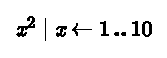
\includegraphics{src/image/for.pdf}
\end{center}

And that's it. In this case, there is some extra effort to enter the \keyword{for}, \keyword{range}, and \keyword{square} nodes. That's the price of being able to add arbitrary nodes to your language. Furthermore, the editor UI could and should be extended to make this penalty as small as possible, for example, since the character `\clojure{f}' has no particular behavior, it could a choice of all known node types beginning with `f'.

These examples hopefully give a sense of how an editor can offer both generality and reasonable usability, but the current \Meta\ editor is certainly only a starting point. Different UI interactions would be appropriate for different kinds of devices (say, emphasizing gestures over keyboard input for a device with a touch-sensitive screen), or for different users (say, something more like a mouse-driven structure editor for end-user programming applications).


%
% Runtime (enumerating the rationals):
%
\section{Using an Extension at Runtime}

In a delightful Functional Pearl\cite{gibbons}, Gibbons et. al present a series of Haskell programs which generate the infinite series of all positive rational numbers. They begin with the idea of traversing the infinite matrix $a_{ij} = i/j$ which contains every positive ratio, but also contains many equivalent, unreduced ratios (e.g. $\nicefrac{1}{2}$, $\nicefrac{2}{4}$, $\dots$).
%$$
%%\left(
%\begin{array}{cccccc}
%\nicefrac{1}{1} & \nicefrac{2}{1} & \nicefrac{3}{1} & \cdots & \nicefrac{m}{1} & \cdots
%\\
%\nicefrac{1}{2} & \nicefrac{2}{2} & \nicefrac{3}{1} & \cdots & \nicefrac{m}{1} & \cdots
%\\
%\vdots
%\\
%\nicefrac{1}{n} & \nicefrac{2}{n} & \nicefrac{3}{n} & \cdots & \nicefrac{m}{n} & \cdots
%\\
%\vdots
%\end{array}
%%\right)
%$$
%Because every integer appears in the denominator in one column and in the numerator in one row, it's apparent that the matrix contains every positive rational. Concatenating the diagonals
%($\nicefrac{1}{1}$), 
%($\nicefrac{1}{2}$, $\nicefrac{2}{1}$), 
%($\nicefrac{1}{3}$, $\nicefrac{2}{2}$, $\nicefrac{3}{1}$), 
%$\cdots$
%gives an infinite series containing all the rationals, and is easily done in constant space. However, this method has two drawbacks in that the rationals are not in reduced form and each equivalent rational is produced many times (for instance, notice that the diagonal $\nicefrac{1}{1}$, $\nicefrac{2}{2}$, $\nicefrac{3}{3}$, $\cdots$ contains only ratios equal to 1).

The authors show that a series containing all positive rationals in reduced form, without duplicates, is obtained by iterating the function 
$x' = 1/{(\lfloor x \rfloor + 1 - \{x\})}$, beginning with $x=1$.\footnote{In the authors' notation, $\lfloor x \rfloor$ is the floor, or whole-number part of $x$, and $\{x\}$ is the fractional part: $\{x\} = x - \lfloor x \rfloor$, $x > 0$.}This is a surprisingly simple expression, but it is somewhat computationally expensive in that calculating $\lfloor x \rfloor$ and $\{x\}$ involves division.

%The series begins:
%\begin{eqnarray*}
%&&1
%\\
%(\lfloor 1 \rfloor + 1 - \{1\})^{-1} 
%= (1 + 1 - 0)^{-1} 
%&=& \nicefrac{1}{2}
%\\
%(\lfloor \nicefrac{1}{2} \rfloor + 1 - \{\nicefrac{1}{2}\})^{-1} 
%= (0 + 1 - \nicefrac{1}{2})^{-1} 
%&=& \nicefrac{2}{1}
%\\ 
%(\lfloor 2 \rfloor + 1 - \{2\})^{-1} 
%= (2 + 1 - 0)^{-1} 
%&=& \nicefrac{1}{3}
%\\ 
%(\lfloor \nicefrac{1}{3} \rfloor + 1 - \{\nicefrac{1}{3}\})^{-1} 
%= (0 + 1 - \nicefrac{1}{3})^{-1} 
%&=& \nicefrac{3}{2}
%\\ 
%(\lfloor \nicefrac{3}{2} \rfloor + 1 - \{\nicefrac{3}{2}\})^{-1} 
%= (1 + 1 - \nicefrac{1}{2})^{-1} 
%&=& \nicefrac{2}{3}
%\\ 
%(\lfloor \nicefrac{2}{3} \rfloor + 1 - \{\nicefrac{2}{3}\})^{-1} 
%= (0 + 1 - \nicefrac{2}{3})^{-1} 
%&=& \nicefrac{3}{1}
%\end{eqnarray*}
Interestingly, this formula can be implemented using only ``a constant number of arbitrary-precision integer additions and subtractions, but no divisions or multiplications'' by choosing a different representation for ratios. This somewhat starting result comes from the fact that the four necessary operations---reciprocal, floor, negate, and fractional part---can all be efficiently performed on ratios represented as \emp{regular continued fractions}. A continued fraction has the form\footnote{Incidentally, this expression is a frequently-cited exception to \TeX's rules for formatting fractions---all the nested expressions are best typeset at the same size, to emphasize the recursive structure. \Meta\ does not provide a way to override that behavior, so continued fractions do not look quite this nice in \Meta!}
$$a_0 + \frac{1}{
    \displaystyle a_1 + \frac{\displaystyle 1}{
        \displaystyle \cdots + \frac{\displaystyle 1}{
            \displaystyle a_n}}}$$
and a regular continued fraction is one in which all the coefficients except $a_0$ are positive, and $a_n > 1$ (except for the special case 1). Every rational has a unique representation as a regular continued fraction.

Having arrived at this elegant result, the authors proceed to reduce their formulas to the notation of Haskell for implementation, using lists of integer coefficients to represent continued fractions. In the process, the origins of the code are completely obscured by the loss of the original notation. For example, one of four cases for negation of a regular continued fraction looks like this\footnote{Actually, what's shown in the paper has been pretty-printed for publication\cite{lhs2tex}. In the actual source code, it must have looked something like this: \clojure{negatecf [n\_0, 2] = [-n\_0-1, 2]}.}:
%$$\mathit{negatecf} (n_0 : 1 : n_2 : ns) = (-n_0 - 1) : (n_2 + 1) : ns$$
%$$-\left(n_0 + \frac{1}{\displaystyle 1 + \frac{1}{n_2 + \cdots}}\right) = (-n_0 - 1) + \frac{1}{(n_2 + 1) + \cdots}$$
$$\mathit{negatecf} [n_0, 2] = [-n_0-1, 2]$$
It's up to the reader (of the paper or of the code) to decode the representation of fractions being used here and work out how this corresponds to the algebra that motivated it. However, in the proper notation, the same definition reads as simple algebraic equation which is easily understood and checked:
$$-\left(n_0 + \frac{1}{2}\right) = (-n_0 - 1) + \frac{1}{2}$$

In \Meta, it's possible to add new syntax which represents the fractions and operations in the the natural way. Because these fractions will be manipulated at runtime, a runtime value is needed to represent them. This can be accomplished by defining a \keyword{continuedFraction} node which expands to an expression constructing a node at runtime. Figure~\ref{fig-cf} shows the resulting declaration, along with some operations provided on the resulting values. The two \clojure{match} nodes provide pattern matching on the runtime shape of the argument, and are used to identify the cases in each operation.

\begin{figure}[h]
  \begin{center}
    
  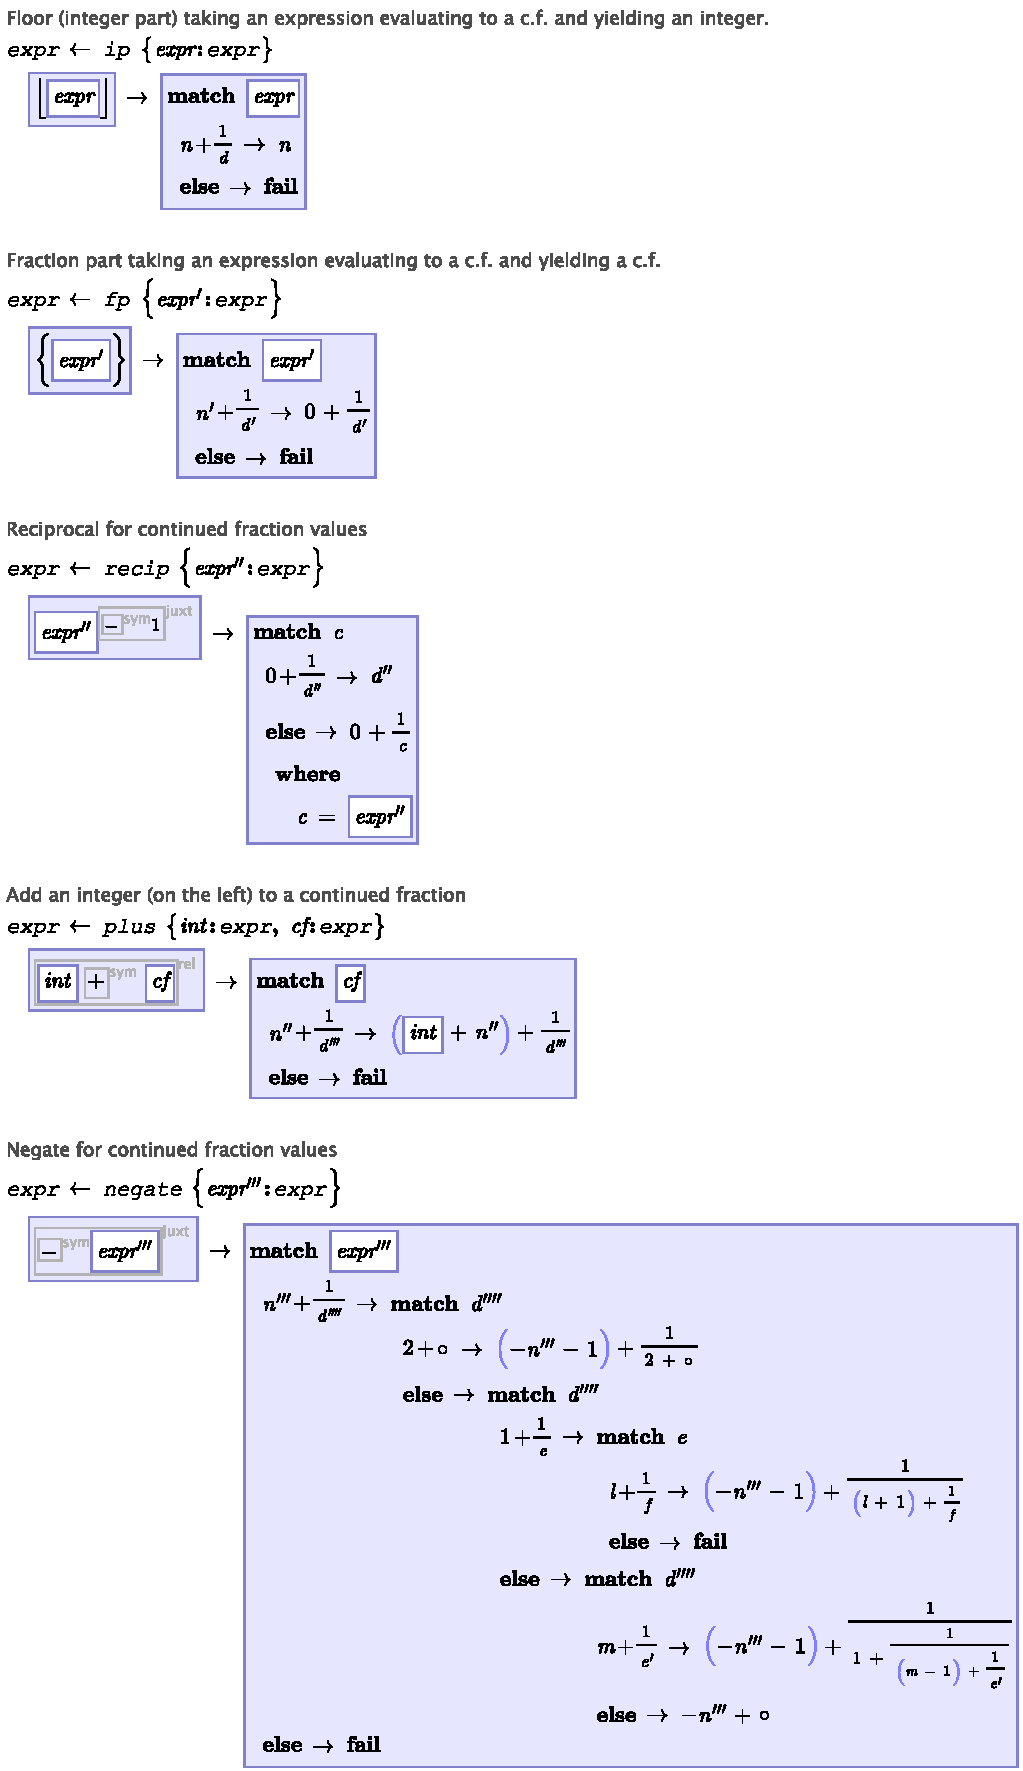
\includegraphics[scale=0.6]{src/image/continued-ops.pdf}
  
  \end{center}
  \caption{Grammar for operations on continued fractions as runtime values.}
  \label{fig-cf}
\end{figure}

Note that these declarations are somewhat straining the current capabilities of \Meta. Ideally the construction of a runtime node would be as simple as adding a second level of quotation to the \keyword{expand} reduction, but the current prototype does not handle that properly, so a bit of extra ceremony is required. Likewise, it would be much more convenient to have a general pattern-match construct supporting multiple patterns, each a node with bindings substituted for one or more of the child nodes, but that is beyond the capabilities of \Meta\ at the moment. However, with the hard work of defining syntax and semantics out of the way, the actual algorithm becomes quite easy to express.

\begin{figure}[h]
  \begin{center}
  
  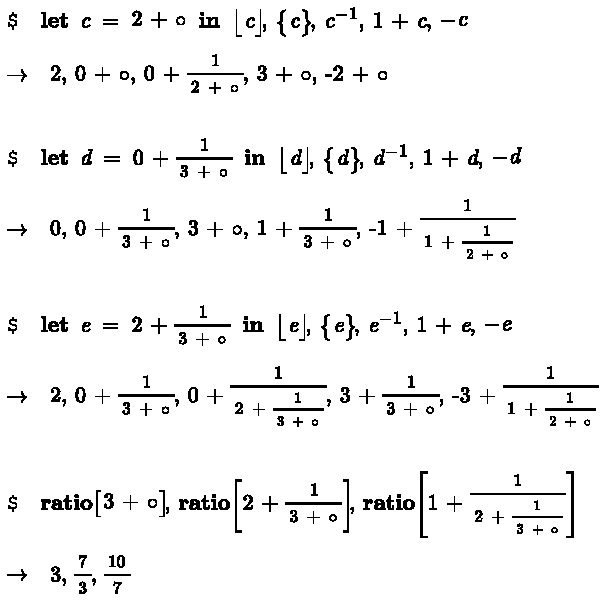
\includegraphics[scale=0.8]{src/image/continued.pdf}
  
%  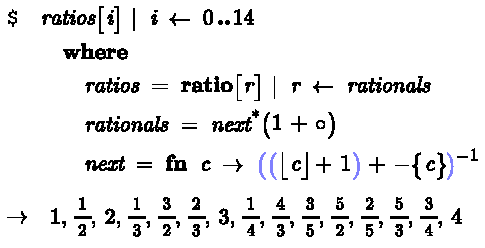
\includegraphics[scale=0.6]{src/image/rationals.pdf}
  
  \end{center}
  \caption{Enumerating the rationals, using continued fractions.}
  \label{fig-cfex}
\end{figure}

\begin{figure}[h]
  \begin{center}
  \todo{capture}
  
  \begin{align*}
  & \mathbf{take}[10, \mathit{rationals}]
  \\
  & \quad \mathbf{where}
  \\
  & \qquad \mathit{ratios} = \mathbf{ratio}[r] ~ | ~ r \leftarrow rationals
  \\
  & \qquad \mathit{rationals} = \mathit{next}^*(1 + \cdot)
  \\
  & \qquad \mathit{next} = \mathrm{fn} ~ c \to \lsyn \lsyn \lfloor c \rfloor + 1 \rsyn + \lsyn -\!\{c\} \rsyn \rsyn^{-1}
  \end{align*}
    
%  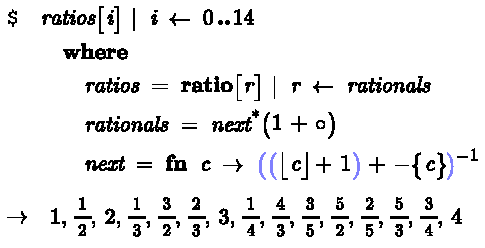
\includegraphics[scale=0.6]{src/image/rationals.pdf}
  
  \end{center}
  \caption{Enumerating the rationals, using continued fractions.}
  \label{fig-rationals}
\end{figure}

With these definitions in hand, the generator for the infinite series of rationals can be written in the proper notation (Figure~\ref{fig-rationals}). The exact form of the expression does not match what was shown earlier because some algrebraic manipulation is necessary to put it into a form that uses only the operations that have been defined. Arguably this is a good thing, because it makes the semantics of the expression explicit.
